\documentclass[10pt,conference,compsocconf]{IEEEtran}

\usepackage{hyperref}
\usepackage{graphicx}	% For figure environment
\usepackage{booktabs}
\usepackage{multirow}
\usepackage{stfloats} % for positioning of figure* on the same page

\begin{document}
\title{Deep Learning Approaches for Mutagenicity Prediction in Chemical Compounds}

\author{
  Jonas-Mika Senghaas, \textit{mika.senghaas@epfl.ch} \\
  \textit{Deep Learning in Biomedicine (CS-502), EPFL, Switzerland}
}

\maketitle

\begin{abstract}

This project explores the use of graph convolutional networks (GCN) to predict
mutagenicity in chemical compounds. Through a rigorous evaluation of various
graph convolutional and pooling techniques on the MUTAG dataset, we have found
that GCNs can effectively learn graph representations, achieving high accuracy
in mutagenicity prediction. The GraphSAGE convolutional layer with sum
aggregation outperforms attention-based and edge graph convolution, with
different pooling operations showing minimal changes in the downstream
performance.

\end{abstract}


\section{Introduction}

Mutagenic compounds have the potential to induce genetic mutations in living
organisms, elevating the risk of cancer. Detecting mutagenicity is thus a
critical endeavour in the field of biomedicine. This project investigates the
capacity of Graph Convolutional Networks (GCNs) with diverse convolutional and
pooling configurations for this purpose. All experiments conducted are fully
reproducible and openly available on
\href{https://github.com/mikasenghaas/cs502}{GitHub}.

\section{Data}

The MUTAG dataset~\cite{mutag} is a popular benchmark dataset for graph
classification in the biomedical domain. It consists of 188 graphs, each
representing a chemical compound with nodes being atoms and edges being bonds.
Both node and edge types are labelled as one of seven atom types and four bond
types, respectively. Each chemical compound is labelled mutagenic (positive
class) or non-mutagenic (negative class). An example of the data is shown in
Figure~\ref{fig:graph} in the Appendix. Table~\ref{tab:dataset} displays
statistics of the entire dataset. The dataset consists of more positive ($66\%$)
than negative examples ($34\%$). Further, all graphs are fully-connected and
small, with an average of $\approx 18$ nodes, $\approx 20$ edges and an average
degree of 2.19. The mutagenic graphs tend to be slightly larger with a higher
average node and edge count. 

\begin{table}[ht]
  \centering
  \begin{tabular}{lccc}
    \toprule
    & \textbf{Overall} & \textbf{Positive} (1)& \textbf{Negative} (0) \\
    \midrule
    \#Graphs & 188 & 125 (66\%) & 63 (34\%) \\
    Avg. \#Nodes & 17.93 & 19.94 & 13.94 \\
    Avg. \#Edges & 19.79 & 22.40 & 14.62 \\
    Avg. Degree & 2.19 & 2.24 & 2.09 \\
    Avg. Connectivity & 1.0 & 1.0 & 1.0 \\
    \bottomrule
  \end{tabular}
  \caption{Dataset Statistics}
  \label{tab:dataset}
\end{table}

\section{Methodology}

The objective is to accurately predict the mutagenicity of chemical compounds by
learning both from the graph's topology and its node and edge features. This
study investigates the potential of graph convolutional networks for this task.
Architecturally, all models are feed-forward graph neural networks that
iteratively update a graph's node feature representation into a meaningful
latent space. To perform the final graph prediction a global pooling operation
maps the node representations to a single graph representation. Finally, a
linear layer with a sigmoid activation function outputs the probability of a
graph being mutagenic. This project explored four different graph convolutional
layers and two global pooling operations, which are introduced in the following.

% TODO: could add a figure here to illustrate the architecture

\subsection{Graph Convolution Layers}

Three of the four graph convolutional layers are well-known methods, including
GraphConv~\cite{graphconv}, GraphSAGE~\cite{graphsage} (with sum aggregation),
and GAT~\cite{gat}. The specifics of the methods are not discussed here. For
details, please refer to the respective papers. The fourth layer is an adapted
version of the edge convolutional EGNN(C) layer, introduced by Gong et
al.~\cite{egnn}. Unlike the other approaches, it incorporates edge features to
update the node representations. The core idea is to treat the edge feature
matrix $\mathbf{E}$ as a collection of $P$ adjacency matrices
$\mathbf{E}_{\cdot\cdot p} \forall p \in P$. Gong et.~al propose to normalise
(Eq.~\ref{eq:row-norm} \&~\ref{eq:col-norm}) the edge feature matrix and then
perform a graph convolution on each of the $P$ channels. The results are then
multiplied element-wise and fed through a non-linear activation function.
However, as the edge features in this dataset are one-hot encoded, the
element-wise product will lead to sparse matrices, which limit the learning
abilities of the model. To counteract this, element-wise summation is used.
Furthermore, each channel is given its own learnable weight matrix
$\mathbf{W}_p$ to allow the model to learn different representations for each
edge type. The layer can be expressed as

\begin{equation}
  \mathbf{H}^{(l+1)} = 
  \sigma\left(
    \sum_{p=1}^P \tilde{\mathbf{E}}_{\cdot\cdot p} \mathbf{H}^{(l)}
    \mathbf{W}^{(l)}_p 
    \right),
\end{equation}

where $\mathbf{W}^{(l)}_p$ is a trainable weight matrix in the $l$-th layer for
the $p$-th channel of the edge feature matrix, $\sigma$ is a non-linear
activation function and $\mathbf{H}^{(l)}$ is the node feature matrix of the
$l$-th layer.


\subsection{Global Pooling Layers}

To obtain a fixed-sized representation of the graph, a global pooling operation
is applied to the latent node representations after the graph convolutional
layers. This study considers the standard mean and max pooling operations.

\section{Experiments}

The study aims to explore the potential of graph convolutional networks for
mutagenicity prediction, as well as the impact of different graph convolutional
and pooling layers on the model's performance. To this end, a grid search was
performed over a set of model and training hyper-parameters. For each
combination of the four graph convolutional layer types (GraphConv, GraphSAGE,
GAT, EdgeConv) and two global pooling layers (Mean, Max), models of varying
sizes were trained and evaluated with varying training hyper-parameters. Model
sizes changed by altering the number of layers ($L \in \{3, 5, 7\}$) and the
hidden units per layer ($H \in \{8, 32, 64\}$). 

All $72$ models were trained using stochastic gradient descent with a batch size
of $1$ for learning rates of $\gamma=\{0.01, 0.001\}$ and a fixed number of
$\eta=100$ epochs. Each model was optimised under weighted, binary cross-entropy
objective using the Adam optimiser~\cite{adam}. A split of $75\%$ is used for
training, $15\%$ for validation and $10\%$ for testing. To obtain a balanced
classifier, model selection is performed based on the validation Macro F1 score
which averages the F1 score over both classes.

\section{Results}

Table~\ref{tab:top5} displays the validation performance of the five best
models. All models achieve a high validation accuracy and Macro F1 score of 
$\sim 90\%$. All models use the GraphSAGE convolutional layer with sum
aggregation. However, the number of layers, hidden units and pooling operation
differ. 

\begin{table}[ht]
  \centering
  \begin{tabular}{lllcccc}
    \toprule
    \multicolumn{5}{c}{\textbf{Parameters}} &
    \multicolumn{2}{c}{\textbf{Validation}} \\
    L & D & $\gamma$ & Conv & Pool & Acc. (\%) & M.-F1 (\%) \\
    \midrule
    5 & 64 & 1e-2 & GraphSAGE & Max & 92.71 & 92.86 \\
    7 & 32 & 1e-2 & GraphSAGE & Max & 89.16 & 89.29 \\
    3 & 32 & 1e-1 & GraphSAGE & Max & 89.16 & 89.29 \\
    3 & 32 & 1e-1 & GraphSAGE & Mean & 88.93 & 89.29 \\
    5 & 64 & 1e-1 & GraphSAGE & Mean & 88.93 & 89.29 \\
    \bottomrule
  \end{tabular}
  \caption{Validation Performance of Top 5 Models}
  \label{tab:top5}
\end{table}

Figure~\ref{fig:scatter-val-f1} shows the validation Macro F1 score of all
models as a function of the number of trainable model parameters. The
convolutional and pooling layer types are encoded through colour and shape,
respectively. In line with the inspection of the top 5 models, the figure shows
that the best performing models are all GraphSAGE models. Interestingly, neither
the attention-based nor the edge convolutional layer are able to reach the same
performance. The training of attention-based models was found to plateau after a
certain number of epochs, which is reflected in the lower validation
performance. The edge convolutional models often overfit to the training data
and not generalise well to the validation data as a result. Further, the
scatter plot does not suggest any clear correlation between the number of
trainable parameters or the pooling operation and the final performance.

\begin{figure}[ht]
  \centering
  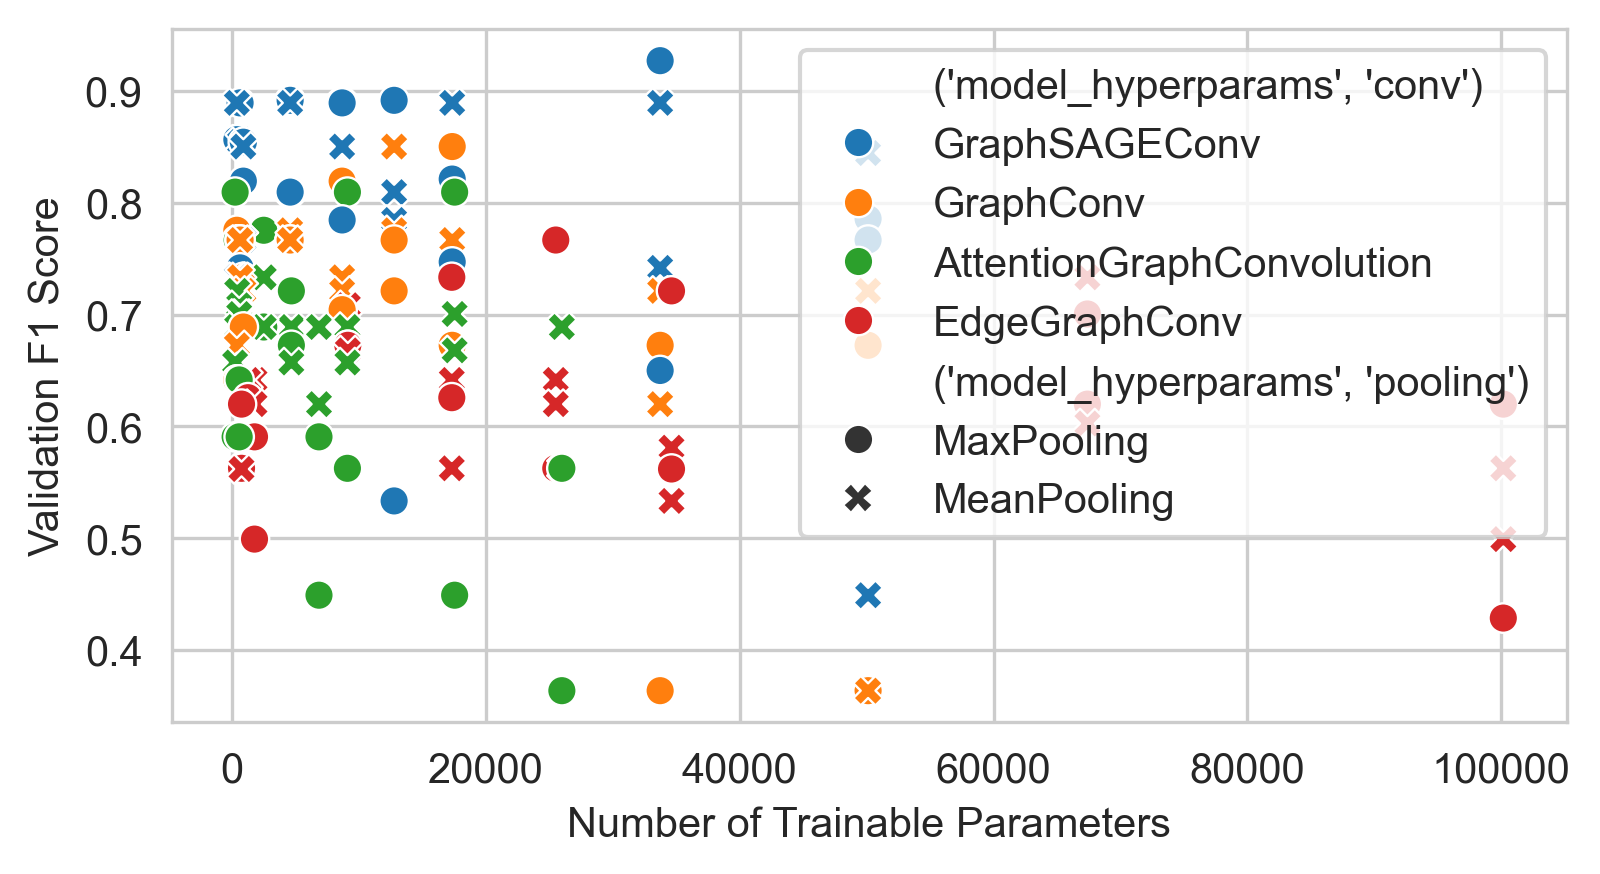
\includegraphics[width=0.45\textwidth]{../plots/scatter-val-f1.png}
  \caption{Validation Macro F1 Score as a function of Model Size}
  \label{fig:scatter-val-f1}
\end{figure}

Figure~\ref{fig:perf_vs_layers} breaks down ``model size'' into the number of
layers and hidden units through a heat map. The figure highlights that more
complex models do not significantly improve performance. The best performing
models are relatively simple with $L=3$ layers and $H=\{32, 64\}$ hidden units.

\begin{figure}[ht]
  \centering
  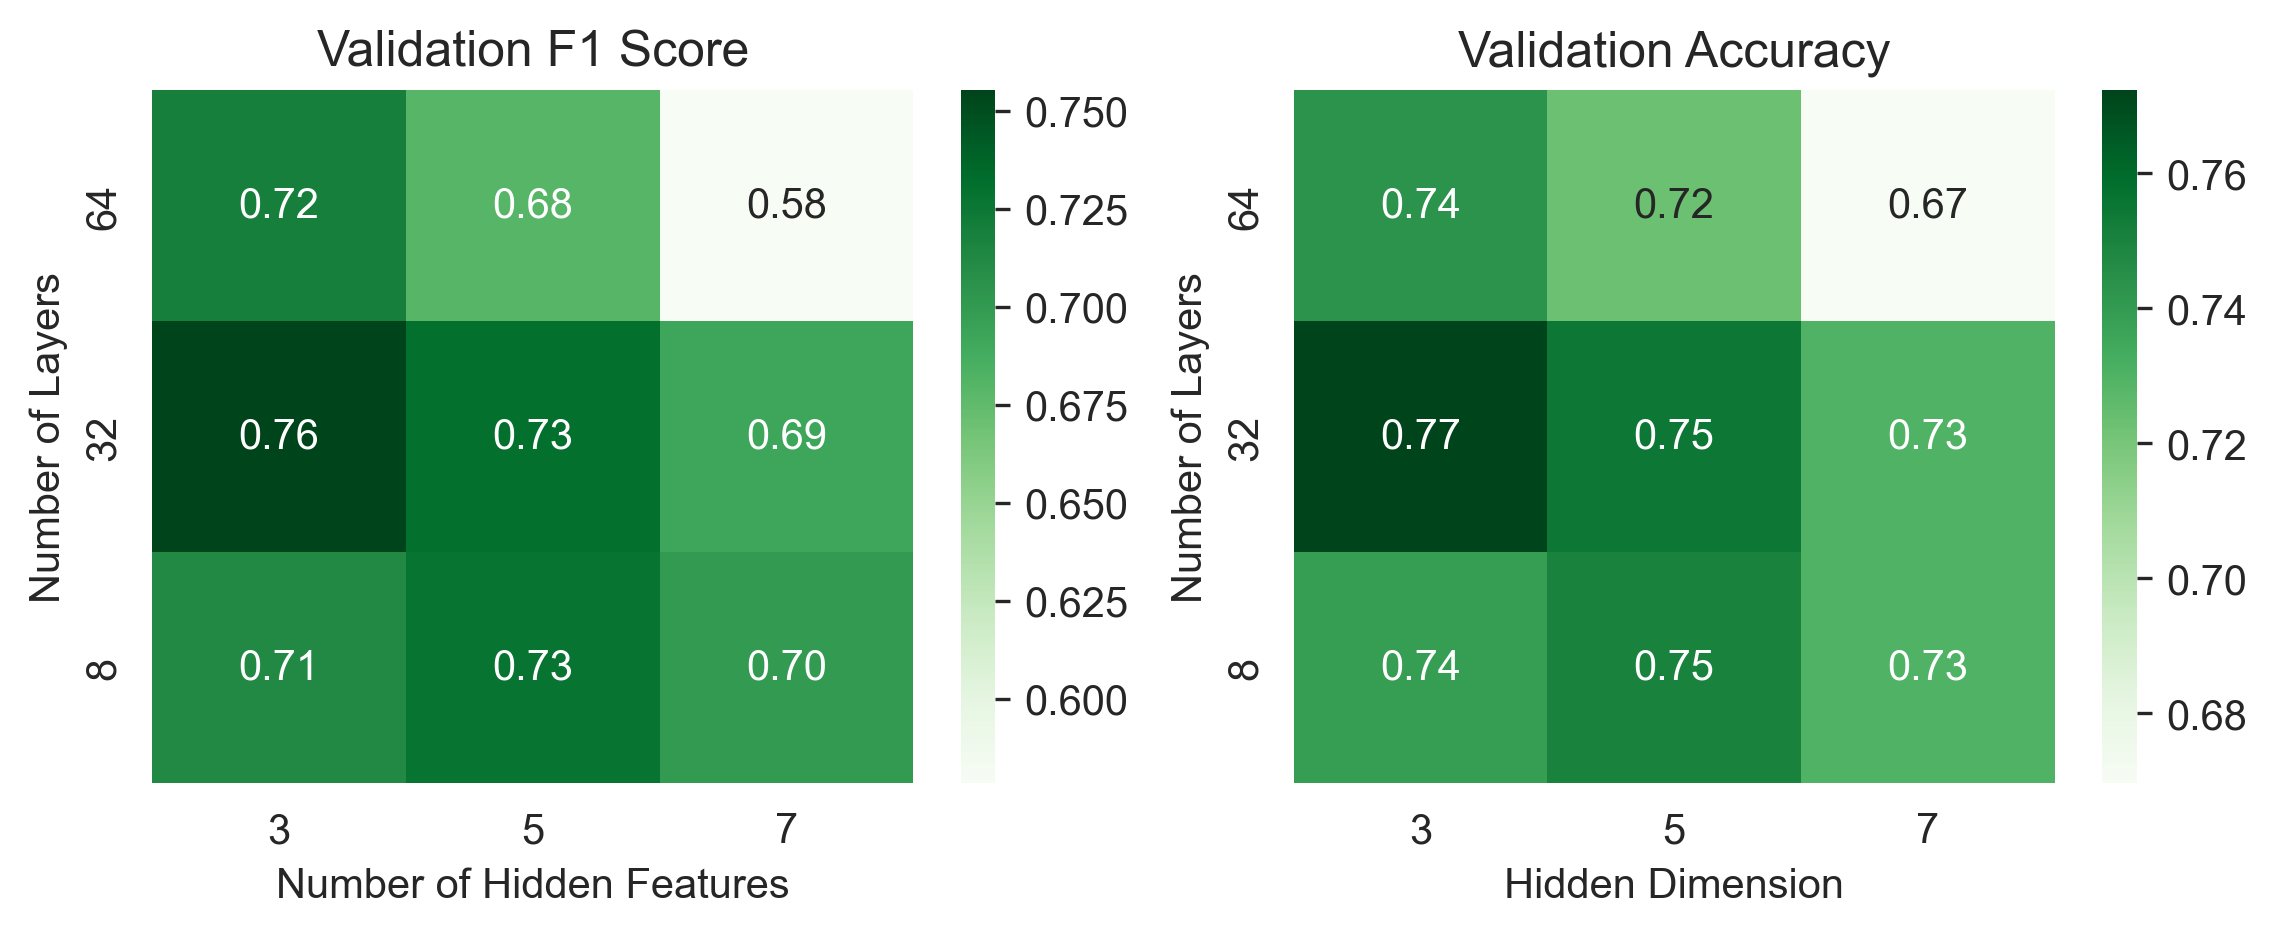
\includegraphics[width=0.45\textwidth]{../plots/heat-val-f1-acc.png}
  \caption{Average Macro F1 Score for Different Numbers of $L$ and $H$}
  \label{fig:perf_vs_layers}
\end{figure}

Finally, evaluating the best-performing model on the test set yields an accuracy
of $\sim\mathbf{89}\%$ and a Macro F1 score of $\sim\mathbf{87}\%$, proving the
model's ability to generalise.

\section{Summary}

The experiments show that graph convolutional networks learn powerful
representations of chemical compounds that allow for accurate prediction of
mutagenicity. Given the small data size, smaller architectures were found to
generalise better and are therefore preferred. The results suggest that the
GraphSAGE layer creates the best models, while the choice of the global pooling
layer does not seem to have a significant impact on the performance.

\newpage
\bibliographystyle{IEEEtran}
\bibliography{literature}

\section{Appendix}

\subsection{Graph Visualisation}

A visualisation of the graph structure of a mutagenic and non-mutagenic graph.
In addition to the graph topology, the plot shows the integer-encoded node and
edge types and denotes the graph's mutagenicity with the node colour.

\begin{figure}[h!]
  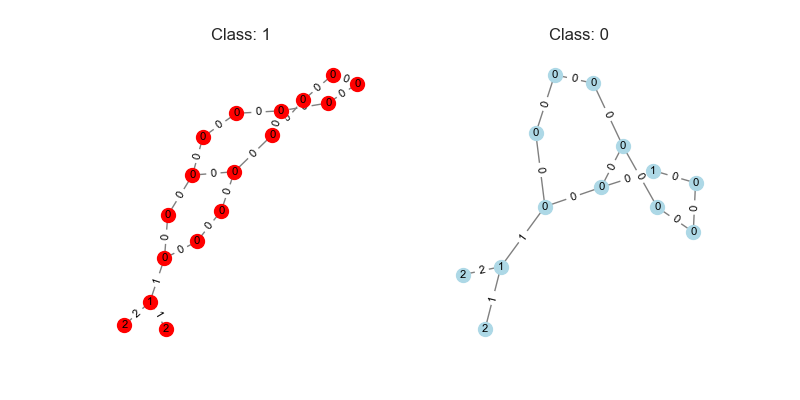
\includegraphics[width=0.48\textwidth]{../plots/graphs.png}
  \caption{Mutagenic vs. Non-Mutagenic Graph}
  \label{fig:graph}
\end{figure}


\begin{figure*}[b]
  \centering
  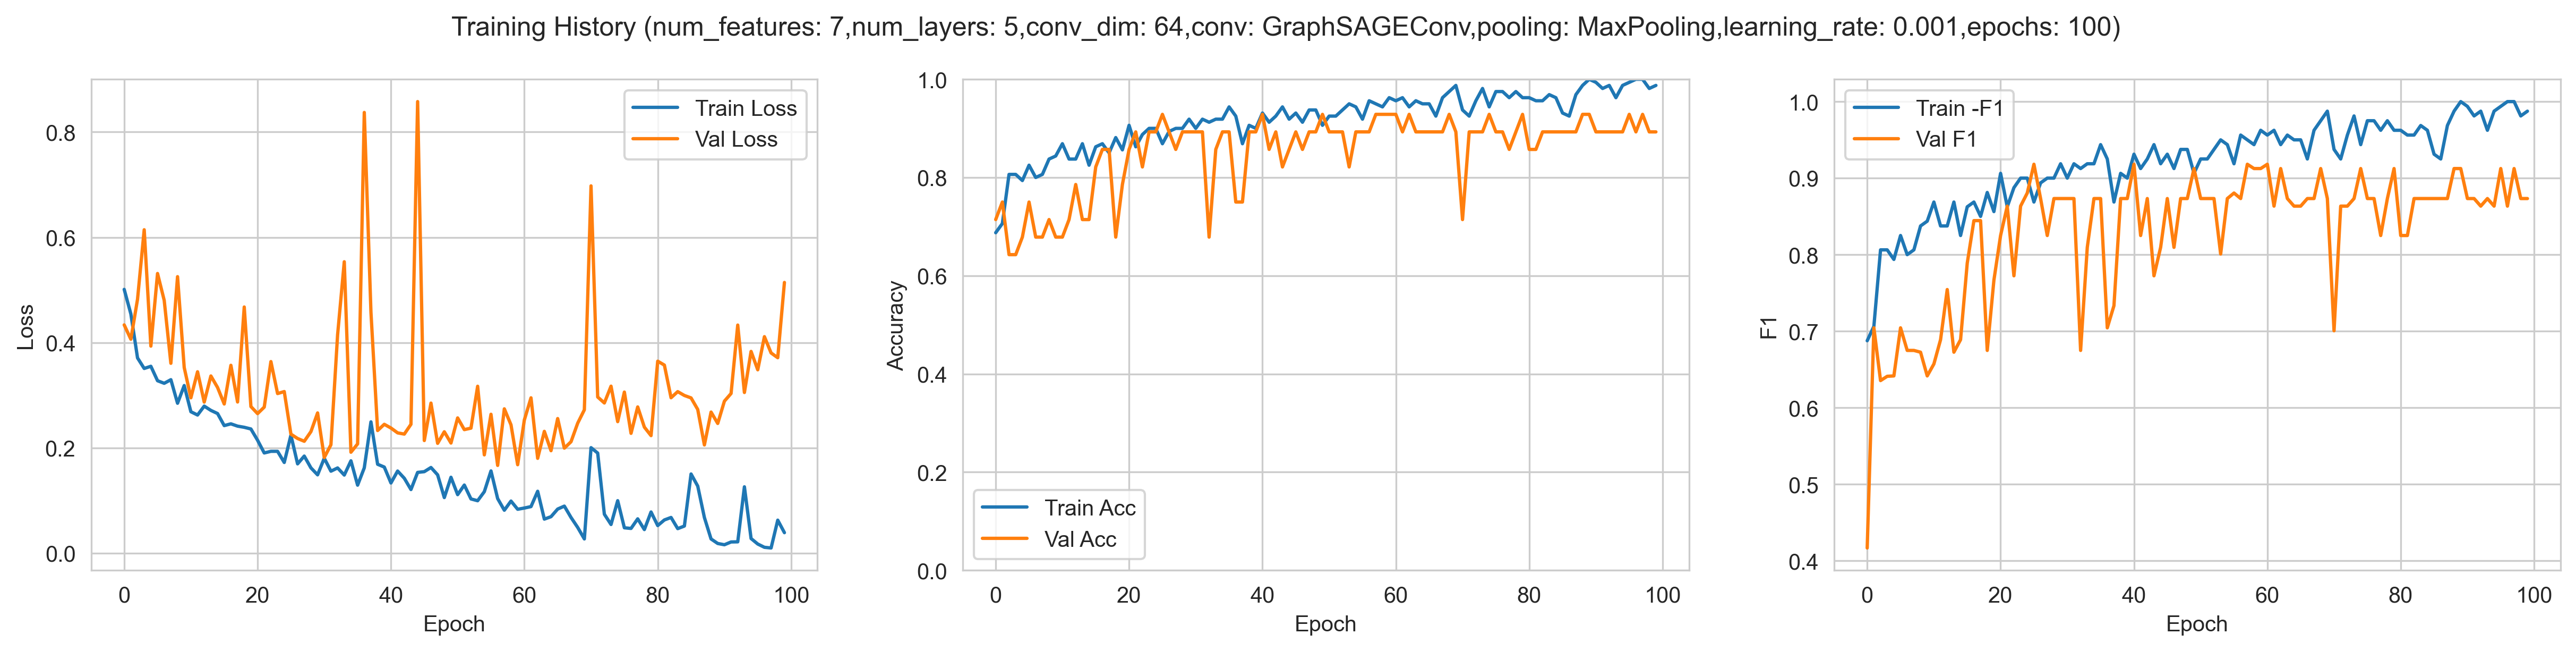
\includegraphics[width=\textwidth]{../plots/training.png}
  \caption{Example Training Curve}
  \label{fig:training}
\end{figure*}

\subsection{Training Curves}

% TODO: figure with training curves for all models
Figure~\ref{fig:training} displays the training curve of the best model when
trained on the full training set. The figure shows the training and validation
loss (left), accuracy (middle) and Macro F1 score (right) over the $\eta = 100$
epochs. The model converges after approximately $50$ epochs.

\subsection{Doubly Stochastic Normalisation}

Gong et al.~\cite{egnn} propose a doubly stochastic normalisation of the edge
feature matrix to prevent the node feature representation from exploding. The
normalisation happens in two steps: The matrix is first normalised row-wise
(Eq.~\ref{eq:row-norm}) and then column-wise (Eq.~\ref{eq:col-norm}). The
resulting matrix is doubly stochastic, i.e.\ the sum of each row and column is
equal to $1$ with all non-negative entries.

\begin{equation}
   \tilde{\mathbf{E}}_{i,j,p} = 
   \frac{\mathbf{E}_{i,j,p}}{\sum_{k=1}^N \mathbf{E}_{ikp}}
   \label{eq:row-norm}
\end{equation}
 
\begin{equation}
  \tilde{\mathbf{E}}_{i,j,p} = 
  \sum_{k=1}^{N}
  \frac{\tilde{\mathbf{E}}_{i,k,p}\tilde{\mathbf{E}}_{j,k,p}}{\sum_{v=1}^N \mathbf{E}_{vkp}}
  \label{eq:col-norm}
\end{equation}

\end{document}
